\documentclass[a4paper, 11pt]{article}

\setcounter{tocdepth}{3}
\setcounter{secnumdepth}{3}

\usepackage{comment} % enables the use of multi-line comments (\ifx \fi) 
\usepackage{lipsum} %This package just generates Lorem Ipsum filler text. 
\usepackage{fullpage} % changes the margin
\usepackage[utf8]{inputenc}
\usepackage{gensymb}
\usepackage{graphicx}
\usepackage{booktabs}% http://ctan.org/pkg/booktabs
\usepackage{makecell}
\usepackage{tabularx}
\usepackage[table]{xcolor}
\usepackage{array}
\usepackage{wrapfig}
\usepackage{subcaption}
\usepackage{csquotes}
\usepackage{lscape}
\usepackage{afterpage}
\usepackage{geometry}
\usepackage{listings}
\usepackage{chngcntr}
\usepackage{multicol}

\counterwithin{figure}{section}

\geometry{a4paper, margin=1in}
\renewcommand{\figurename}{Abb.}
\renewcommand{\tablename}{Tabelle}
\newcommand{\code}[1]{\texttt{#1}}

\renewcommand*{\thead}[1]{\bfseries #1}

\renewcommand{\contentsname}{Inhalt}
\renewcommand{\listfigurename}{Abbildungsverzeichnis}


\begin{document}
 
\title{Einführung in die Internationalen Beziehungen - HS2018}
\author{Alex Neher}
\maketitle

\tableofcontents
\newpage
\listoffigures
\newpage

\graphicspath{{./Pictures/}}


\section{Einführung}
\subsection{Definitionen}
\subsubsection{Politikwissenschaft}
Die Definition der Politikwissenschaften hat sich mit der Zeit verändert:
\begin{description}
    \item[Traditionell:] Handlungen des Staates und seiner Organe verstehen
    \item[Modern:] Breites Verständnis des Politischen aneignen
    \item[Heute:] Das Zusammenspiel zwischen Staat und Gesellschaft verstehen
\end{description}        

\vspace{10px}
\noindent Die heutige Politiwissenschaft lässt sich in verschiedene Subkategorien unterteilen:
\begin{multicols}{2}
    \begin{itemize}
        \item Das Politische System
        \item Vergleichende Politikwissenschaften
        \item Internationale Beziehungen
\columnbreak
        \item Politische Theorie
        \item Methodenlehre
        \item Politisches Verhalten
    \end{itemize}
\end{multicols}

Man geht davon aus, dass jeder Bürger zumindest ein Grundverständnis der Politik und der politischen Zusammenhänge hat. Der Unterschied zwischen diesem Grundwissen (Allgemeinwissen) und der Politikwissenschaft ist, dass die Politikwissenschaft \textit{auf systematische Art und Weise logisch konsistente, falsifizierbare und gleichzeitig empirisch bestätigte} Aussagen erarbeitet, während es auch als politisches Allgemeinwissen aufgefasst werden kann, wenn man sagt "Hillary Clinton hätte die Präsidentschaftswahl gewonnen, wenn man sich nicht auf die E-Mails konzentriert hätte." Denn diese Aussage ist weder falsifizierbar (man weiss nicht, ob es tatsächlich stimmt) noch ist sie empirisch bestätigt (es gibt keine Referenzwerte, die diese Aussage bestätigen oder eben falsifizieren würden)

\vspace{10px }

\noindent Es gibt \textbf{vier} Kriterien der politikwissenschaftlichen Forschung: 

\begin{description}
	\item[Inferenz: ] Schlussfolgerung über den Einzelfall hinaus. \\
	Ein Einzelfall ist nichts wert. Es müssen möglichst viele Beobachtungen präsentiert werden, die diese These unterstützen.
	\item[Methodik: ] Der Unterschied zwischen wissenschaftlichen Aussagen und Meinungen ist, dass bei Meinungen die Methode nicht zwingend nachvollziehbar (oder überhaupt vorhanden) sein muss, während bei wissenschaftlichen Aussagen die verwendete Methodik öffentlich zugänglich und nachvollziehbar sein muss.
	\item[Verwandte Methodik: ] Wissenschaftliche Aussagen sollten wenn immer möglich mit einer bereits verwendeten und 'anerkannten' Methodik durchgeführt werden, was auch die Nachprüfung der Aussage vereinfacht.
	\item[Schlussfolgerungen: ] Schlussfolgerungen sind zwar unsicher, der Grad/das Ausmass der Unsicherheit ist jedoch abschätzbar \\
	Man kann zwar nicht mit Sicherheit sagen, dass der neue Präsident mit exakt 80\% Wähleranteil gewählt wird, aber man kann davon ausgehen, dass es 80\% $\pm$ 5\% sein wird.
\end{description}

\subsubsection{Theorie vs. Modell}

\begin{tabularx}{\textwidth}{p{7cm}p{7cm}} 
	\textbf{Theorie} &  \textbf{Modell}\\ 
		\blockquote{Abstrahierende und verallgemeinernde Betrachtung und Auseinandersetzung mit der Wirklichkeit} & \blockquote{Eine Vereinfachte Darstellung der Wirklichkeit, um wesentliche Dinge besser zu verstehen} \\
		  & Eine Menge von vereinfachenden Annahmen und daraus ableitbaren Aussagen über einen Zusammenhang \\ 
\end{tabularx}

\vspace{10px}

So kann ein Modell z.B. eine Karte sein: Sie zeigt eine vereinfachte Darstellung der Wirklichkeit (Die Welt, vereinfacht in 2D). Ausserdem werden nur die wichtigen Dinge wie z.b. der Bahnhof dargestellt, während unwichtige Dinge weggelassen werden. 

\paragraph{Arten von Theorien} \mbox{} \\
Es wird zwischen drei Haupttypen von Theorien unterschieden: 

\begin{description}
	\item[Deskriptiv: ] \textit{Was ist das Wesentliche eines Phänomens?} \\
	"Was macht die Staatenwelt aus?"
	\item[Normativ: ] \textit{Wie sollte eine ideale Welt aussehen?} \\
	"Hat die NATO das Recht zur Intervention in souveränen Staaten?"
	\item[Empirisch-analytisch: ] \textit{Wie sieht die tatsächliche Welt aus?} - Fokus auf Erklärung politischer Prozesse/Events \\
	"Wieso hat Trump die US-Wahlen gewonnen?"
\end{description}

\subsubsection{Politik}
Der Begriff 'Politik' ist folgendermassen definiert:

\begin{center}
    \blockquote{Soziales Handeln, das auf Entscheidungen und Steuerungsmechanismen ausgerichtet ist, die allgemein verbindlich sind und das Zusammenleben von Menschen regeln.}
\end{center}

Die Politik lässt sich grundsätzlich in drei Arten unterteilen. In der Deutschen Sprache werden für alle drei Begriffe dasselbe Wort verwendet, im Englischen kann jedoch unterschieden werden zwischen: 
\begin{description}
    \item[Policy: ] \textit{Was} - Inhalte der Politik. Regeln, Weisungen
    \item[Polity:] \textit{Wer} - Die Strukturen und Akteure der Politik.  Organisationen, Parteien 
    \item[Politics:]  \textit{Wie} - Die Prozesse, wie Regeln, Weisungen etc. entstehen.
\end{description}

\subsubsection{Staat}
Ein Staat benötigt laut dem Völkerrecht mind. die folgenden drei Elemente, um als Staat anerkannt zu werden: 
\begin{description}
    \item[Staatsgebiet: ] Ein Gebiet, über welches der Staat die alleinige Macht hat
    \item[Staatsvolk: ] Ein Volk, welches im Staatsgebiet lebt und unter der Staatsgewalt des Staates ist.
    \item[Staatsgewalt: ] Der Staat hat das Recht, Gesetze zu erlassen und diese durchzusetzen. Er darf Steuern erlassen, um öffentliche Güter bereitzustellen oder Einkommen umzuverteilen. Jedoch muss der Staat die innere und äussere Sicherheit garantieren können.
\end{description}

\begin{figure}[htb]
    \centering
    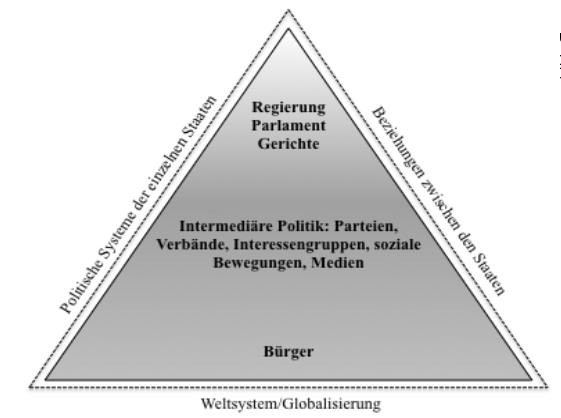
\includegraphics[keepaspectratio=true,height=15\baselineskip]{analytische_grundstruktur.png}
    \caption{Grundstruktur eines Staates}
    \label{fig:grundstrk_staat}
\end{figure}

Die Interessen der Staatsbürger werden meist über sogenannte \textit{Intermediärorgane} gewahrt. Das sind z.B. Parteien, Organisationan o.ä; Kurz gesagt, Polity.

\newpage

\subsection{Internationale Beziehungen}

Durch das Studium von internationalen Beziehungen versucht man zu verstehen, wie verschiedene Völker miteinander umgehen und miteinander auskommen. Die untersuchten Beziehungen können sowohl von freundschaftlicher, wie aber auch von kriegerischer Natur sein.

\vspace{10px}

Schimmelfennig beschreibt die internationale Politik als \blockquote[Schimmelfennig 2015, p.19]{Gesamtheit aller Interaktionen, die auf die autoritative Verteilung von Werten jenseits staatlicher Grenzen gerichtet sind}. Soll heissen; Alle Bemühungen, eine internationale Gesellschaft aufzubauen, die nach ähnlichen oder den gleichen Werten strebt.

\vspace{10px}

Im Gegensatz zur nationalen Politik, in welcher es eine Regierung in irgendeiner Form (Parlament, König o.ä) gibt, herrscht in der internationalen Politik \textbf{Anarchie}. Es gibt \textbf{keine zentrale Autorität} im internationalen System. Jegliche Allianzen und Kooperationen die zwischen Staaten existieren sind selbstbestimmt. Sie bleiben nur solange bestehen, wie der stärkere der beiden Staaten einen Gewinn daraus ziehen kann.

Diese Anarchie im internationalen Umfeld stellt die einzelnen Staaten je nach dem vor schwer zu lösende Probleme. Prinzipiell sind es dieselben Probleme, die sie auch staatsintern zu meistern haben, jedoch herrscht dort keine Anarchie (oder sollte zumindest nicht)

Grundsätzlich lassen sich diese Probleme in drei Hauptkategorien unterteilen:


\begin{description}
	\item[Sicherheit: ] Es gibt keine zentrale Autorität, die das Gewaltsmonopol hat, wie das in der inneren Politik der Fall ist. Jeder Staat muss selbst für seine Sicherheit sorgen.
	
	
	Das heisst, entweder findet ein Wettrüsten a la Kalter Krieg statt, oder aber man muss Allianzen eingehen. Diese Allianzen halten aber auch nur so lange, wie der stärkere Allianzpartner etwas davon hat.
	\item[Wohlfart: ] Aufgrund dessen, dass es keine zentrale Autoritätsstelle 	gibt, sind die internationalen Märkte enorm fragmentiert. Jeder Staat ist auf seinen eigenen Vorteil bedacht. Es werden nationale Währungen herausgegeben, Zölle für Import und Export erhoben und der grenzüberschreitende Warenaustausch wird von beiden Staaten streng überwacht. \\
	All das lässt sich mit einem Wort zusammenfassen: \textit{\textbf{ineffizient}}. Es gibt einen enormen bürokratischen Overhead und treiben die Preise in die Höhe, da die ganze Bürokratie irgendwie finanziert werden müsste.
	
	
	Im schlimmsten Fall kann dies zu Marktversagen führen. Marktversagen tritt dann auf, wenn Angebot und Nachfrage nicht mehr im Verhältnis stehen und somit zu massiv niedrigeren Preisen verkauft werden muss und somit Verluste eingefahren werden.
	
	\item[Freiheit: ] Die Bürger und Bürgerinnen eines jeden Staates geniessen gewisse Freiheiten innerhalb ihres Staates (idealerweise Meinungsfreiheit, Freiheit vor Folter, Verfolgung etc.). Diese Freiheiten sind jedoch an ihren jeweiligen Heimatstaat gebunden.
	
	
	Diese Freiheiten können sich je nach Herrschaft eines Staates enorm unterscheiden (man denke an die Unterschiede Schweiz vs. Nordkorea). Es müssen also Abmachungen getroffen und Verträge ausgehandelt werden, dass die Bürger aller Staaten in allen anderen Staaten vergleichbare Rechte geniessen.
\end{description}

\section{Realismus und Neo-Realismus}



\subsection{Analyseebenen}
Die Politik kann auf verschiedenen Ebenen analysiert werden:

\begin{description}
	\item[Individuum: ] Die persönliche Einstellung von Individuen wird analysiert
	\item[Regierung: ] Ds Verhalten von Regierungen wird analysiert.
	\item[Gesellschaft: ]
	\item[Zwischenmenschlich: ]
	\item[Weltsystem: ]
\end{description} 
\end{document}
